\documentclass[a4paper,12pt]{ctexart}
\usepackage{geometry}
\usepackage{amsmath, amssymb, amstext}
\usepackage{graphicx}
\usepackage{xcolor}
\usepackage{float}
\usepackage{tikz}
\usepackage{pgfplots}
\usepackage{enumitem}
\usepackage{cases}
\usepackage{tcolorbox}
\usepackage[UTF8]{ctex} % 中文支持
\usepackage{amsmath, amssymb}
\usepackage{geometry}
\geometry{a4paper, scale=0.8}
\usepackage{float} % 支持 [H]
\usepackage{tikz}
\usepackage{pgfplots}

\pgfplotsset{compat=1.18} % 推荐的 pgfplots 配置
\geometry{left=2.0cm, right=2.0cm, top=2.5cm, bottom=2.5cm}

% 定义颜色以匹配原��
\definecolor{myorange}{RGB}{235, 120, 50}
\definecolor{myblue}{RGB}{70, 115, 200}
\definecolor{highlightred}{RGB}{200, 30, 30}
\definecolor{notepurple}{RGB}{230, 230, 250}
\definecolor{myblue}{RGB}{0, 114, 189}
\definecolor{highlightred}{RGB}{217, 83, 25}
\definecolor{myorange}{RGB}{237, 177, 32}
% 定义紫色框环��
\newenvironment{purplebox}
  {\begin{tcolorbox}[colback=white, colframe=purple, boxrule=1pt, sharp corners]}
  {\end{tcolorbox}}

% 定义绿色框环��
\newenvironment{greenbox}
  {\begin{tcolorbox}[colback=white, colframe=green!60!black, boxrule=1pt, sharp corners]}
  {\end{tcolorbox}}

% 定义zh命令用于中文段落
\newcommand{\zh}[1]{\par\smallskip\noindent#1\par\smallskip}

\title{\textbf{考研数学-高数总结(冲刺�?)}}
\author{}
\date{}

\begin{document}

\maketitle
\section*{初等数学公式}

\subsection*{常见的三角函数图像}

\begin{figure}[H]
    \centering
    \begin{minipage}{0.48\textwidth}
        \centering
        \begin{tikzpicture}[scale=0.7]
            \begin{axis}[
                axis lines=middle,
                xmin=-4.9, xmax=4.9,
                ymin=-3.5, ymax=3.5,
                xtick={-4.71, -3.14, -1.57, 1.57, 3.14, 4.71},
                % 修复：去掉了奇怪的 \\end{cases} 乱码
                xticklabels={$\frac{3\pi}{2}$, $\pi$, $\frac{\pi}{2}$, $\frac{\pi}{2}$, $\pi$, $\frac{3\pi}{2}$},
                ytick={-1, 1, 2, 3},
                grid=both,
                major grid style={line width=.2pt,draw=gray!30},
                width=\linewidth,
                height=0.8\linewidth,
                tick label style={font=\tiny},
                clip=true
            ]
                % sin(x)
                \addplot[domain=-4.9:4.9, samples=100, color=myblue, thick] {sin(deg(x))};
                \node[color=myblue, font=\tiny] at (axis cs: 2.5, 0.8) {$\sin(x)$};
                
                % cos(x)
                \addplot[domain=-4.9:4.9, samples=100, color=highlightred, thick] {cos(deg(x))};
                \node[color=highlightred, font=\tiny] at (axis cs: 1.2, 0.8) {$\cos(x)$};
                
                % tan(x)
                \addplot[domain=-1.4:1.4, samples=50, color=myorange, thick] {tan(deg(x))};
                \addplot[domain=1.74:4.5, samples=50, color=myorange, thick] {tan(deg(x))};
                \addplot[domain=-4.5:-1.74, samples=50, color=myorange, thick] {tan(deg(x))};
                \node[color=myorange, font=\tiny] at (axis cs: -1.0, 2.5) {$\tan(x)$};
                
            \end{axis}
            \node[font=\scriptsize, below] at (current bounding box.south) {正弦、余弦以及正切函数};
        \end{tikzpicture}
    \end{minipage}
    \hfill
    \begin{minipage}{0.48\textwidth}
        \centering
        \begin{tikzpicture}[scale=0.7]
             \begin{axis}[
                axis lines=middle,
                xmin=-2.2, xmax=2.2,
                ymin=-1.8, ymax=3.5,
                xtick={-2, -1, 1, 2},
                ytick={-1.57, 1.57, 3.14},
                % 修复：去掉了奇怪的 \\end{cases} 乱码
                yticklabels={$-\frac{1}{2}\pi$, $\frac{1}{2}\pi$, $\pi$},
                grid=both,
                major grid style={line width=.2pt,draw=gray!30},
                width=\linewidth,
                height=0.8\linewidth,
                tick label style={font=\tiny}
            ]
                % arcsin
                \addplot[domain=-1:1, samples=100, color=myblue, thick] {rad(asin(x))};
                \node[color=myblue, font=\tiny, anchor=west] at (axis cs: 1.1, 1.0) {$\arcsin(x)$};
                
                % arccos
                \addplot[domain=-1:1, samples=100, color=highlightred, thick] {rad(acos(x))};
                \node[color=highlightred, font=\tiny, anchor=east] at (axis cs: -0.5, 2.8) {$\arccos(x)$};
                
                % arctan
                \addplot[domain=-2.2:2.2, samples=100, color=myorange, thick] {rad(atan(x))};
                \node[color=myorange, font=\tiny, anchor=west] at (axis cs: 1.1, 0.5) {$\arctan(x)$};
                
                \draw[dashed, gray] (axis cs:-2, 1.57) -- (axis cs:2, 1.57);
                \draw[dashed, gray] (axis cs:-2, -1.57) -- (axis cs:2, -1.57);
            \end{axis}
            \node[font=\scriptsize, below] at (current bounding box.south) {反正弦、反余弦以及反正切函数};
        \end{tikzpicture}
    \end{minipage}
\end{figure}

\subsection*{常见的三角函数公式}

\textbf{六角形法则}

\begin{figure}[H]
    \centering
    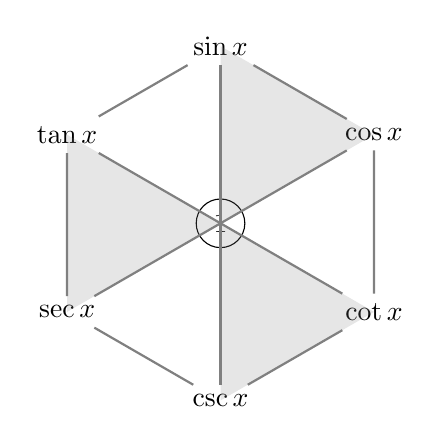
\begin{tikzpicture}[scale=1.5]
        % 修复：去掉了节点文字周围的 \\end{cases}
        % Hexagon vertices
        \node (sin) at (90:1.5) {$\sin x$};
        \node (cos) at (30:1.5) {$\cos x$};
        \node (cot) at (-30:1.5) {$\cot x$};
        \node (csc) at (-90:1.5) {$\csc x$};
        \node (sec) at (-150:1.5) {$\sec x$};
        \node (tan) at (150:1.5) {$\tan x$};
        \node[circle, draw, fill=white] (one) at (0,0) {1};

        % Edges
        \draw[thick, gray] (sin) -- (cos) -- (cot) -- (csc) -- (sec) -- (tan) -- (sin);
        
        % Diagonals
        \draw[thick, gray] (sin) -- (csc);
        \draw[thick, gray] (cos) -- (sec);
        \draw[thick, gray] (tan) -- (cot);
        
        % Shading
        \fill[gray, opacity=0.2] (0,0) -- (90:1.5) -- (30:1.5) -- cycle;
        \fill[gray, opacity=0.2] (0,0) -- (-30:1.5) -- (-90:1.5) -- cycle;
        \fill[gray, opacity=0.2] (0,0) -- (-150:1.5) -- (150:1.5) -- cycle;
    \end{tikzpicture}
\end{figure}

\newpage

\section*{常用三角函数公式}

\[ \cos^2 x + \sin^2 x = 1 \quad \cos^2 x - \sin^2 x = \cos 2x \]

\[ 2\sin x \cos x = \sin 2x \]

\[ 1 - \cos 2x = 2\sin^2 x \quad 1 + \cos 2x = 2\cos^2 x \]

\[ 1 + \tan^2 x = \frac{1}{\cos^2 x} = \sec^2 x \quad 1 + \cot^2 x = \frac{1}{\sin^2 x} = \csc^2 x \]

\[ \sin x \sin y = -\frac{1}{2}[\cos(x+y) - \cos(x-y)] \]

\[ \cos x \cos y = \frac{1}{2}[\cos(x+y) + \cos(x-y)] \]

\[ \sin x \cos y = \frac{1}{2}[\sin(x+y) + \sin(x-y)] \]

\section*{和差化积公式}

\begin{align*}
    \sin \alpha + \sin \beta &= 2\sin\frac{\alpha+\beta}{2}\cos\frac{\alpha-\beta}{2} \\
    \sin \alpha - \sin \beta &= 2\cos\frac{\alpha+\beta}{2}\sin\frac{\alpha-\beta}{2} \\
    \cos \alpha + \cos \beta &= 2\cos\frac{\alpha+\beta}{2}\cos\frac{\alpha-\beta}{2} \\
    \cos \alpha - \cos \beta &= -2\sin\frac{\alpha+\beta}{2}\sin\frac{\alpha-\beta}{2}
\end{align*}
*(注：原文最后一个公式系数为 $2\sin...$，但标准公式应包含负号或调整顺序，此处依据原文截图看似有负号或书写习惯，标准为$-2\sin\sin$)*

\section*{倍角公式}

\begin{align*}
    \sin 2\alpha &= 2\sin \alpha \cos \alpha \\
    \cos 2\alpha &= 2\cos^2 \alpha - 1 = 1 - 2\sin^2 \alpha = \cos^2 \alpha - \sin^2 \alpha \\
    \cot 2\alpha &= \frac{\cot^2 \alpha - 1}{2\cot \alpha} \\
    \tan 2\alpha &= \frac{2\tan \alpha}{1 - \tan^2 \alpha}
\end{align*}

\begin{align*}
    \sin 3\alpha &= 3\sin \alpha - 4\sin^3 \alpha \\
    \cos 3\alpha &= 4\cos^3 \alpha - 3\cos \alpha \\
    \tan 3\alpha &= \frac{3\tan \alpha - \tan^3 \alpha}{1 - 3\tan^2 \alpha}
\end{align*}

\section*{三角形诱导公式}

\noindent\textbf{口诀：}奇变偶不变（对于 $n$ 而言），符号（对于 $x + n \cdot \frac{\pi}{2}$）看象限。
将$\sin(x + n \cdot \pi/2)$ 中的 $x$ 看作是锐角。

\vspace{0.5cm}
\noindent\textbf{手写笔记补充（反三角函数与三角函数嵌套及其他）：}

\begin{itemize}
    \item \textbf{补充公式：}
    \[ \arctan x + \arctan \frac{1}{x} = \begin{cases} \frac{\pi}{2}, & x > 0 \\ -\frac{\pi}{2}, & x < 0 \end{cases} \]
    
    \item \textbf{嵌套化简：}
    \[ \arcsin(\sin t) = \begin{cases} t, & t \in [0, \frac{\pi}{2}] \\ \pi - t, & t \in [\frac{\pi}{2}, \frac{3\pi}{2}] \end{cases} \]
    
    \item \textbf{六边形推论（倒数关系）：}
    \[ \csc x = \frac{1}{\sin x}, \quad \sec x = \frac{1}{\cos x}, \quad \cot x = \frac{1}{\tan x} \]
    \[ \tan x = \frac{\sin x}{\cos x}, \quad \cot x = \frac{\cos x}{\sin x} \]
    
    \item \textbf{平方关系：}
    \[ \sin^2 x + \cos^2 x = 1, \quad 1 + \tan^2 x = \sec^2 x, \quad 1 + \cot^2 x = \csc^2 x \]
    
    \item \textbf{诱导公式补充（配角公式）：}
    \[ \sin(x) = \cos(\frac{\pi}{2} - x) \]
    \[ \arctan x + \arctan \frac{1}{x} = \text{const} \]
    \[ \arcsin x + \arccos x = \frac{\pi}{2} \]
\end{itemize}

\section*{反三角函数与三角函数嵌套}

\noindent \textbf{反三角函数常识：}
\begin{enumerate}
    \item 当$x \in [0, \pi]$ 时，$\arccos[\cos x] = x$。
          当$x \in [-\pi, 0]$ 时，$\arccos[\cos x] = -x$ （此处原文手写推导，意为利用偶函数性质）。
    \item 当$x \in [-\frac{\pi}{2}, \frac{\pi}{2}]$ 时，$\arcsin(\sin x) = x$。
    \item 当$x \in (-\frac{\pi}{2}, \frac{\pi}{2})$ 时，$\arctan(\tan x) = x$。
          当$x \in \mathbb{R}$时，$\tan(\arctan x) = x$。
\end{enumerate}

\section*{数列求和公式}

\textbf{等比数列求和公式：}
\[ S_n = \frac{a_1(1-q^n)}{1-q} = \frac{a_1 - a_n q}{1-q} \quad (q \neq 1) \]
\[ S_n = n a_1 \quad (q = 1) \]

\textbf{等差数列求和公式：}
\[ S_n = \frac{n(a_1 + a_n)}{2} = n a_1 + \frac{n(n-1)d}{2} \]

\vspace{0.5cm}
\noindent\textbf{手写笔记补充（数列技巧）：}
\begin{enumerate}
    \item 等差数列通项公式为：$a_n = a_1 + (n-1)d$。
    \item $n$ 项和为：$S_n = \frac{n}{2}[2a_1 + (n-1)d]$。
    \item 等比数列通项公式为：$a_n = a_1 q^{n-1}$。
          求和为：$S_n = \frac{a_1(1-q^n)}{1-q}$。
    \item 常用的一堆数列求和结论：
          \begin{itemize}
              \item $\sum_{k=1}^n k = 1 + 2 + 3 + \cdots + n = \frac{n(n+1)}{2}$
              \item $\sum_{k=1}^n k^2 = 1^2 + 2^2 + 3^2 + \cdots + n^2 = \frac{n(n+1)(2n+1)}{6}$
              \item $\sum_{k=1}^n \frac{1}{k(k+1)} = \frac{1}{1\times 2} + \frac{1}{2\times 3} + \cdots + \frac{1}{n(n+1)} = \frac{n}{n+1}$ (裂项相消)
          \end{itemize}
\end{enumerate}

\section*{面积、体积公式}

\begin{itemize}
    \item 长方体的表面积 = (长 × 宽 + 长 × 高 + 宽 × 高) × 2
    \item 长方体的体积 = 长 × 宽 × 高 \quad $V = abh$
    \item 正方体的表面积 = 棱长 × 棱长 × 6 \quad $S = 6a^2$
    \item 正方体的体积 = 棱长 × 棱长 × 棱长 \quad $V = a^3$
    \item 圆柱的侧面积 = 底面圆的周长 × 高 \quad $S = ch$
    \item 圆柱的表面积 = 上下底面面积 + 侧面积
    \item $S = 2\pi r^2 + 2\pi rh = 2\pi(r+h)$
    \item 圆柱的体积 = 底面积 × 高 \quad $V = Sh$
    \item \fbox{$V = \pi r^2 h = \pi (d ÷ 2)^2 h$}
    \item 圆锥的体积 = 底面积 × 高 ÷ 3
    \item \fbox{$V = Sh ÷ 3 = \pi r^2 h ÷ 3$}
    \item 长方体（正方体、圆柱体）的体积 = 底面积 × 高 \quad $V = Sh$
\end{itemize}

\section*{距离公式}

\subsection*{点到点}
两点 $P(x_1, y_1), Q(x_2, y_2)$ 间的距离为：
\[ \sqrt{(x_1 - x_2)^2 + (y_1 - y_2)^2} \]
\small{分析：把两点放到平面直角坐标系中，连接两点作为对角线，分别过两点作平行于坐标轴的直线...，相信已经很明显了，出现了直角三角形，由勾股定理得出结论。}

\subsection*{点到直线}
设$P(x_0, y_0)$ 到直线$Ax + By + C = 0, \quad (A^2 + B^2 \neq 0)$ 的距离为
\[ \frac{|Ax_0 + By_0 + C|}{\sqrt{A^2 + B^2}} \]

\subsection*{直线到直线}
\textbf{两条平行直线}
\[ Ax + By + C_1 = 0 \]
\[ Ax + By + C_2 = 0 \]
间的距离为：
\[ \frac{|C_1 - C_2|}{\sqrt{A^2 + B^2}} \]

\subsection*{点到平面}
设$M(x_0, y_0, z_0)$ 是平面$Ax + By + Cz + D = 0, \quad (A^2 + B^2 + C^2 \neq 0)$ 外一点，则该点到该平面的距离为：
\[ \frac{|Ax_0 + By_0 + Cz_0 + D|}{\sqrt{A^2 + B^2 + C^2}} \]

\section*{一元二次方程}

\[ ax^2 + bx + c = 0 \]
\[ a(x + \frac{b}{2a})^2 - \frac{b^2}{4a} + c = 0 \]
\[ (x + \frac{b}{2a})^2 = \frac{b^2 - 4ac}{4a^2} \]
\[ x + \frac{b}{2a} = \pm \frac{\sqrt{b^2 - 4ac}}{2a} \]
\[ x = \frac{-b \pm \sqrt{\Delta}}{2a}, \quad \Delta = b^2 - 4ac \]

其中 $\Delta = b^2 - 4ac$ 决定了方程能否顺利完成开平方的运算，被称为根的判别式。
\begin{itemize}
    \item 如果 $\Delta > 0$，那么我们就能顺利开平方，计算出 $x$ 的两个解，也可以叫两个根。
    \item 而如果 $\Delta < 0$，我们不能对负数开平方，方程在实数范围内无解。
    \item 特别地，$\Delta = 0$ 时，我们说方程的两个解大小一样，叫做重根。
\end{itemize}

\section*{二次函数的两根式}

如果函数 $f(x) = ax^2 + bx + c$ 对应的方程$ax^2 + bx + c = 0$ 有两个根，分别是 $x = x_1, x = x_2$，那么我们可以得到二次函数的另一种写法：
\[ f(x) = a(x - x_1)(x - x_2) \]
两个根代入后满足函数值为0的条件，且是一个二次项系数为$a$ 的二次函数。
这种写法被叫做二次函数的两根式。

\section*{韦达定理}

\[ f(x) = a(x - x_1)(x - x_2) = ax^2 - a(x_1 + x_2)x + ax_1 x_2 = ax^2 + bx + c \]
比较两者的各项系数，很容易得到：
\[ -a(x_1 + x_2) = b, \quad ax_1 x_2 = c \]
\fbox{$\begin{cases} x_1 + x_2 = -\frac{b}{a}, \\ x_1 x_2 = \frac{c}{a} \end{cases}$}

两个根的和与乘积直接通过方程系数计算，这就是韦达定理。
由于两根式只有在方程可解的情况下才有，所以实数范围内的韦达定理需要首先计算根的判别式，从而判断方程是否可解。

\section*{二项式定理}

$(a+b)^n = C_n^0 a^n + C_n^1 a^{n-1}b + \cdots + C_n^k a^{n-k}b^k + \cdots + C_n^n b^n \quad (n \in N^*)$ 等号右边的多项式叫做 $(a+b)^n$ 的二项展开式，其中各项的系数$C_n^k (k=0,1,2,3 \cdots n)$ 叫做二项式系数。

\[ a^n - b^n = (a-b)(a^{n-1} + a^{n-2}b + \cdots + ab^{n-2} + b^{n-1}) \]

\section*{立方和差公式}

\begin{enumerate}
    \item $a^3 - b^3 = (a-b)(a^2 + ab + b^2)$
    \item $a^3 + b^3 = (a+b)(a^2 - ab + b^2)$
\end{enumerate}

% Page 1 Content
\noindent
3.
\[ (a-b)^3 = a^3 + 3ab^2 - 3a^2b - b^3 \]
\[ (a+b)^3 = a^3 + 3ab^2 + 3a^2b + b^3 \]

\end{document}